\documentclass[conference]{IEEEtran}
\usepackage{blindtext, graphicx}
\usepackage[spanish]{babel}
\usepackage{skmath}
\usepackage[utf8]{inputenc}
\usepackage{amsmath}
\usepackage{amsfonts}
\usepackage{graphicx}
\usepackage[colorinlistoftodos]{todonotes}
\usepackage{algorithm}
\usepackage{algpseudocode}
\usepackage{pgfplots}
\pgfplotsset{width=9cm,compat=1.9}
\graphicspath{ {C:/Users/CASA/Pictures} }

\begin{document}
\title{$ I$ Primer Proyecto Programado Insta AA}
\author{\IEEEauthorblockN{Daniel Alvarado Bonilla}
\IEEEauthorblockA{Instituto Tecnol\'ogico de Costa Rica\\Ingenier\'ia en Computaci\'on\\
2014089192\\
Email: daniel.alvarado.bonilla@gmail.com}
\and
\IEEEauthorblockN{Roberto Rojas Segnini}
\IEEEauthorblockA{Instituto Tecnol\'ogico de Costa Rica\\Ingenier\'ia en Computaci\'on\\
2016139072\\
Email:rojassegniniroberto@gmail.com}
}
\maketitle
\begin{abstract}
%\boldmath
%\blindtext[1]
The present paper intends to clarify and explain the performance, efficiency and importance of an algorithm, in this particular case, algorithms used in image Filters. \\ There are two kinds of algortihms used, the first kind creates black and white filters, and the other apply image convulsion to create different effects. \\Besides the explaining made , the time execution of each algorithm is described and analyzed. Also, experiments were made so that there is a empiric explanation of the time duration of the algorithms. \\The reader may be able to learn the Big O of the algorithms implemented in the project, the algorithms complexity and the importance of using most effective algorithm.
\end{abstract}
\begin{IEEEkeywords}
O Grande, Matriz, Algoritmo.
\end{IEEEkeywords}
\section{Introducci\'on}
Intro
\section{Pseudoc\'odigo}
  \begin{algorithm}
   \caption{Average Algorithm}
    \begin{algorithmic}[1]
      \Function{avergingImage}{Bitmap bitmap }\\\Comment{Donde Bitmap es el el array de pixeles utilizados para programar en Android}
		\\
        \State int color, red, blue, green, newColor;
        \State  Bitmap image $= bitmap.copy(Bitmap.$
        \State $Config.ARGB8888, true)$
\\
        \For{$y = 0$ to image height}
            \For{$x = 0$ to image width}
            		\State color = image.getPixel(y,x)
            		\State blue = Color.blue(color)
            		\State green = Color.green(color)
            		\State red = Color.red(color)
            		\State newColor $= ((red+green+blue)/3)*0x00010101$
                \State image.setPixel(x, y, newColor)
        		\EndFor
        \EndFor
        \State return image
       \EndFunction

\end{algorithmic}
\end{algorithm}
\begin{algorithm}
   \caption{Decomposition Max Algorithm}
    \begin{algorithmic}[1]
      \Function{decompositionMax}{Bitmap bitmap }\\\Comment{Donde Bitmap es el el array de pixeles utilizados para programar en Android}
		\\
        \State int color, red, blue, green, newColor;
        \State  Bitmap image $= bitmap.copy(Bitmap.$
        \State $Config.ARGB8888, true)$
\\
        \For{$y = 0$ to image height}
            \For{$x = 0$ to image width}
            		\State color = image.getPixel(y,x)
            		\State blue = Color.blue(color)
            		\State green = Color.green(color)
            		\State red = Color.red(color)
            		\State newColor $= ((Math.max(Math.max(red, green), blue)))*0x00010101$
                \State image.setPixel(x, y, newColor)
        		\EndFor
        \EndFor
        \State return image
       \EndFunction

\end{algorithmic}
\end{algorithm}
\begin{algorithm}
   \caption{Decomposition Min Algorithm}
    \begin{algorithmic}[1]
      \Function{decompositionMin}{Bitmap bitmap }\\\Comment{Donde Bitmap es el el array de pixeles utilizados para programar en Android}
		\\
        \State int color, red, blue, green, newColor;
        \State  Bitmap image $= bitmap.copy(Bitmap.$
        \State $Config.ARGB8888, true)$
\\
        \For{$y = 0$ to image height}
            \For{$x = 0$ to image width}
            		\State color = image.getPixel(y,x)
            		\State blue = Color.blue(color)
            		\State green = Color.green(color)
            		\State red = Color.red(color)
            		\State newColor $= ((Math.min(Math.$
            		\State $min(red, green), blue)))*0x00010101$
                \State image.setPixel(x, y, newColor)
        		\EndFor
        \EndFor
        \State return image
       \EndFunction

\end{algorithmic}
\end{algorithm}
\begin{algorithm}
   \caption{Desaturation Algorithm}
    \begin{algorithmic}[1]
      \Function{desaturation}{Bitmap bitmap }\\\Comment{Donde Bitmap es el el array de pixeles utilizados para programar en Android}
		\\
        \State int color, red, blue, green, newColor;
        \State  Bitmap image $= bitmap.copy(Bitmap.$
        \State $Config.ARGB8888, true)$
\\
        \For{$y = 0$ to image height}
            \For{$x = 0$ to image width}
            		\State color = image.getPixel(y,x)
            		\State blue = Color.blue(color)
            		\State green = Color.green(color)
            		\State red = Color.red(color)
            		\State newColor $= (((Math.max(Math.max$
            		\State$(red, green), blue) + Math.min(Math.min(red, green),$
                    \State $blue))/2) *0x00010101)$
                \State image.setPixel(x, y, newColor)
        		\EndFor
        \EndFor
        \State return image
       \EndFunction

\end{algorithmic}
\end{algorithm}
\begin{algorithm}
   \caption{Gaussian Algorithm}
    \begin{algorithmic}[1]
      \Function{GaussianFilter}{Bitmap bitmap }\\\Comment{Donde Bitmap es el el array de pixeles utilizados para programar en Android}
		\\
        \State int color, blue, green, red, sumBlue = 0, sumGreen = 0,				 \State sumRed = 0;
        \State  Bitmap image $= bitmap.copy(Bitmap.$
        \State $Config.ARGB8888, true)$
\\
		\State $int[ ][ ] kernel =$
          \State ${1, 4, 7, 4, 1},$
          \State ${4, 16, 26, 16, 4},$
                        \State ${7, 26, 41, 26, 7},$
                       \State $ {4, 16, 26, 16, 4},$
                        \State ${1, 4, 7, 4, 1} $
                        \\
                        \\
         \State int imgH $= image.getHeight(); $
        \State int imgW $= image.getWidth(); $
       \State int kerL $= kernel.lenght; $
        
\\
        \For{$int y = 1;y<imgH-kL;y=y+1$}
            \For{$int x = 1;y<imgW-kL;x++$}
				\For{$int v= 0; v < kL; v++$}
					\For{$int u= 0; u < kL; u++$}
						\State color$= image.getPixel(x+u,y+v)$
						\State blue = Color.blue(color)
            				\State green = Color.green(color)
            				\State red = Color.red(color)
            				\State sumGreen $+= (green)*kernel[u][v]$
            				\State sumBlue $+= (blue)*kernel[u][v]$
            				\State sumRed $+= (red)*kernel[u][v]$
            			\EndFor
				\EndFor
				\State sumGreen $=sumGreen/kernelSum$
				\State sumBlue $=sumBlue/kernelSum$
				\State sumRed $=sumRed/kernelSum$
				\State newImg = $ setPixel(x, y, $				
				\State Color.setRGB(Math.abs(sumRed), 
				\State Math.abs(sumGreen), Math.abs(sumBlue)));
        		\EndFor
        \EndFor
        \State return image
       \EndFunction

\end{algorithmic}
\end{algorithm}
\begin{algorithm}
   \caption{Sobel Operator Algorithm}
    \begin{algorithmic}[1]
      \Function{desaturation}{Bitmap bitmap }
		\\
        \State int color, blue, green, red, sumBlue = 0, sumGreen = 0,				 \State sumRed = 0;
        \State  Bitmap image $= bitmap.copy(Bitmap.$
        \State $Config.ARGB8888, true)$
\\
		\State $int[ ][ ] kernel =$
          \State ${-1, 0, 1},$
          \State ${-2, 0, 2}$
                        \State ${-1, 0, 11},$
                        \\
                        \State $int[ ][ ] kernel2 =$
          \State ${-1, -2, -1},$
          \State ${0,0,0},$
                        \State ${1,2,1},$
                        \\
                        \\
         \State int imgH $= image.getHeight(); $
        \State int imgW $= image.getWidth(); $
       \State int kerL $= kernel.lenght; $
        
\\
        \For{$int y = 1;y<imgH-kL;y=y+1$}
            \For{$int y = 1;y<imgW-kL;x++$}
            \State $sumGrey = 0, sumGrey2 = 0$
				\For{$int v= 0; v < kL; v++$}
					\For{$int u= 0; u < kL; u++$}
						\State color$= image.getPixel(x+u,y+v)$
						\State blue = Color.blue(color)
            				\State green = Color.green(color)
            				\State red = Color.red(color)
            				\State color $= (red+green+blue)/3$
            				\State sumGrey $+= (color) * kernel[u][v]$
            				\State sumGrey2 $+= (color) * kernel2[u][v]$
            			\EndFor
				\EndFor
				\State double gradient1 
				\State $=$ Math.sqrt(Math.pow(sumGrey2, 2)
				\State$+$Math.pow(sumGrey, 2));
				\State newImg = $ setPixel(x, y,  (int)gradient1<<16 | $ 
				\State $(int)gradient1<<8 | (int)gradient1)$
        		\EndFor
        \EndFor
        \State return newImg
       \EndFunction

\end{algorithmic}
\end{algorithm}

\section{Complejidad de los Algoritmos}
Orden de $O(f(n))$ del Filtro Gaussiano:\\
Este algoritmo, tiene en el, cuatro iteraciones de tipo $for$. Donde se, utilizan tres variables diferentes. Las ultimas dos iteraciones, utilizan la misma. Esta, podria considerarse constante ya que siempre usa el mismo tamaño (el kernel nunca cambia) pero para efectos del $O(f(n))$ se considero como una variable.  Al utilizar un $for$, siempre se tiene el siguiente orden: $1 + (n+1) + n$.  Cuando se hace el $int y = 1$ es una constante c, luego la comparacion se hace $n+1$ veces y por \'ultimo, se aumenta la variable $n$ veces. Bas\'andose en lo dicho anterior, el algoritmo se divide en cuatro partes $P$. La primera $P_1$ la dicha anteriormente, donde es la iteracion de mas afuera. El $P_2$ es el segundo $for$, el cual es del tamaño del ancho de la im\'agen. Y el \'ultimo, se podr\'ia decir que es $P_3(k)$, siendo k el tamaño del kernel utilizado. Se considera que donde ocurre el mayor tiempo de ejecuci\'on de operaciones es en $P_2$ y $P_3(k)$. El orden $P_2$ es: $P_3(k) x nc + nc + nc + nP_4 
$, este $P_4$ es la funci\'on encargada de cambiar el pixel de la nueva imagen, donde se considera una constante $c$.  La parte $P_3(k) $ tiene dos ciclos internos (for) donde dependen de la varaible $k $, esta representa el tamaño del kernel utilizado para la convulusi\'on. Al analizar todo el algoritmo y no solo los bucles por separado, se considera que el orden de O grande es $O(n^4)$ al existir cuatro diferentes ciclos, donde dependen de la entrada, la cual, es la im\'agen a utilizar. \\
\\
Orden de $O(f(n))$ de Algoritmos de Blanco y Negro:\\
Estos algoritmos tiene un orden de $nxn$, por lo tanto $n^2$. Esto es deducido por que se recorre cada pixel de la im\'agen. Al ser una matriz de pixeles, tiene un comportamiento cuadratico, aunque la imagen no puede ser cuadrada y seria $mxn $ debe considerarse como una sola entrada, por lo tanto $n^2$.
\\Si se quiere de una forma mas especifica, estos algoritmos de Decomp. Min y Max, Desaturation Y Averaging, difieren uno de otro por las constantes que ocurren adentro del segundo bucle, que para efectos del orden O grande, se consideran irrelevantes. Estas constantes son ciertamente donde se diferencian los algoritmos, ya que es donde suceden las operaciones matem\'aticas. No cambia el orden porque estas constantes, son operaciones elementales, como asignaciones y operaciones matem\'aticas. 



\section{Experimentos}
\subsection{Experimento 1}
El objetivo es determinar el impacto que tiene el tamaño de la imagen
sobre el tiempo requerido para aplicar el filtro. Para esto, se utilizarán
imágenes 10x10, 100x100, 500x500, 750x750 y 1000x1000. El filtro se aplica diez veces,
para determinar un promedio fidedigno en milisegundos del tiempo requerido para aplicar
el filtro. \newline

Como los algoritmos requieren recorrer la imagen, pixel por pixel, para efectuar los cambios
en los valores, es de esperarse que el tiempo requerido sea mayor según aumenta el tamaño de
la foto. Según la teoría, en el peor de los caso se recorre la imagen nxm veces, donde n y m son
el largo y el ancho de la imagen. En nuestro caso, al ser cuadradas, el peor de los caso se define
como $n^2$.\newline

De este modo, en una imagen 10x10 se requieren $10^2=100$ iteraciones; en una 100x100, 10000; en una 500x500, 250000; en una 750x750, 562500; y en una 1000x1000, 1000000 iteraciones. Como vemos, la diferencia entre el número de iteraciones es significativa entre una imagen y otra. En algunos casos la diferencia es alrededor de mil veces mayor.\newline
Tomando como base lo anterior, a continuación se muestran los resultados obtenidos al aplicar
los filtros a imágenes con tamaños diferentes. Los tiempos están dados en milisegundos. En el caso de los gráficos, los milisegundos aparecen escritos en notación científica.\newline


Tiempos de ejecución según tamaño de imagen.

\subsubsection{Averaging}

.
\newline

10x10\newline
1,2,1,1,1,1,2,4,1,2.\newline
Promedio: 1.6
\newline

100x100\newline
10, 126, 93, 114, 114, 110, 113, 110, 115, 90.\newline
Promedio: 99.5
\newline

500x500\newline
2382, 2331, 2361, 2348, 2400, 2426, 2347, 2294, 2391, 2413.\newline
Promedio: 2369.3
\newline

750x750\newline
5368, 5347, 5572, 5440, 5495, 5455, 5325, 5396, 5347, 5542.\newline
Promedio: 5428.7
\newline

1000x1000\newline
10074, 9912, 9974, 9691, 10086, 10167, 9952, 9923, 10002, 9806.\newline
Promedio: 9958.7\newline

\begin{tikzpicture}
\begin{axis}[
    title={Averaging},
    ylabel={Tamaño de la imagen (pixeles)},
    xlabel={Tiempo de ejecución (milisegundos)},
    xmin=0, xmax=11000,
    ymin=0, ymax=1000,
    xtick={0, 1.6, 99.5, 2369.3, 5428.7, 9958.7},
    ytick={0, 10,100,500,750,1000},
    legend pos=north west,
    ymajorgrids=true,
    grid style=dashed,
    width=8.5cm
]
 
\addplot[
    color=blue,
    mark=square,
    ]
    coordinates {
    (1.6, 10)(99.5,100)(2369.3, 500)(5428.7, 750)(9958.7, 1000)
    };
    %\legend{CuSO$_4\cdot$5H$_2$O}
 
\end{axis}
\end{tikzpicture}
\newline

\subsubsection{Desaturation}

.
\newline

10x10\newline
2, 1, 2, 1, 2, 1, 1, 2, 1.\newline
Promedio: 1.3
\newline

100x100\newline
134, 130, 126 126, 155, 158, 124, 127, 148, 128.\newline
Promedio: 135.6 
\newline

500x500\newline
3268, 3422, 3482, 3580, 3374, 3465, 3489, 3414, 3639, 3515.\newline
Promedio: 3811.7
\newline

750x750\newline
7794, 7832, 7918, 7817, 7784, 8051, 7918, 7735, 7220, 7613.\newline
Promedio: 7768.2
\newline

1000x1000\newline
13646, 14112, 13681, 14058, 13714, 13390, 13561, 13919, 13894, 13746.\newline
Promedio: 13772.1\newline
\begin{tikzpicture}
\begin{axis}[
    title={Desaturation},
    ylabel={Tamaño de la imagen cuadrada (pixeles)},
    xlabel={Tiempo de ejecución (milisegundos)},
    xmin=0, xmax=15000,
    ymin=0, ymax=1000,
    xtick={0, 1.3, 135.6, 3811.7, 7768.2, 13772.1},
    ytick={0, 10,100,500,750,1000},
    legend pos=north west,
    ymajorgrids=true,
    grid style=dashed,
    width=9cm%,height=3cm
]
 
\addplot[
    color=blue,
    mark=square,
    ]
    coordinates {
    (1.3, 10)(135.6,100)(3811.7, 500)(7768.2, 750)(13772.1, 1000)
    };
    %\legend{CuSO$_4\cdot$5H$_2$O}
 
\end{axis}
\end{tikzpicture}



\subsubsection{Decomposition max}
.
\newline

10x10\newline
2, 1, 1, 2, 7, 1, 2, 1, 1, 1.
\newline
Promedio: 1.9
\newline

100x100\newline
146, 107, 105, 132, 118, 113, 115, 113, 134, 107.
\newline
Promedio: 119 
\newline

500x500\newline
2793, 2923, 3064, 3037, 3045, 2972, 2968, 2817, 2910, 2927.
\newline
Promedio: 2945.6
\newline

750x750\newline
6625, 6928, 6772, 6787, 6736, 6775, 6457, 6831, 6961, 6494.
\newline
Promedio: 6736.6
\newline

1000x1000\newline
11647, 12037, 11723, 12179, 11685, 11816, 11969, 12086, 12085.
\newline
Promedio: 10722.7\newline
\begin{tikzpicture}
\begin{axis}[
    title={Decomposition max},
    ylabel={Tamaño de la imagen cuadrada (píxeles)},
    xlabel={Tiempo de ejecución (milisegundos)},
    xmin=0, xmax=11000,
    ymin=0, ymax=1000,
    xtick={0, 1.9, 119, 2945.6, 6736.6, 10722.7},
    ytick={0, 10,100,500,750,1000},
    legend pos=north west,
    ymajorgrids=true,
    grid style=dashed,
    width=9cm
]
 
\addplot[
    color=blue,
    mark=square,
    ]
    coordinates {
    (1.9, 10)(119,100)(2945.6, 500)(6736.6, 750)(10722.7, 1000)
    };
    %\legend{CuSO$_4\cdot$5H$_2$O}
 
\end{axis}
\end{tikzpicture}



\subsubsection{Decomposition min}

.
\newline

10x10\newline
2, 1, 2, 1, 1, 1, 2, 2, 2, 1.
\newline
Promedio: 1.5
\newline

100x100\newline
112, 109, 145, 107, 106, 131, 133, 109, 108, 108.
\newline
Promedio: 116.8 
\newline

500x500\newline
2950, 3025, 287, 3040, 2903, 2956, 2997, 3048, 3072.
\newline
Promedio: 2427.8
\newline

750x750\newline
6674, 7013, 6794, 6683, 6616, 6756, 6748, 6699, 6839.
\newline
Promedio: 6082.2
\newline

1000x1000\newline
11998, 11979, 12142, 11951, 11781, 12109, 11864, 12069, 11772.
\newline
Promedio: 10766.5\newline
\begin{tikzpicture}
\begin{axis}[
    title={Decomposition min},
    ylabel={Tamaño de la imagen (pixeles)},
    xlabel={Tiempo de ejecución (milisegundos)},
    xmin=0, xmax=11000,
    ymin=0, ymax=1000,
    xtick={0, 1.5, 116.8, 2427.8, 6082.2, 10766.5},
    ytick={0, 10,100,500,750,1000},
    legend pos=north west,
    ymajorgrids=true,
    grid style=dashed,
    width=9cm
]
 
\addplot[
    color=blue,
    mark=square,
    ]
    coordinates {
    (1.5, 10)(116.8,100)(2427.8, 500)(6082.2, 750)(10766.5, 1000)
    };
    %\legend{CuSO$_4\cdot$5H$_2$O}
 
\end{axis}
\end{tikzpicture}



\subsubsection{Comparaciones}

Es claro que el tamaño de la imagen tiene un impacto relevante en el tiempo
de los algoritmos. Este impacto es de notable extensión, aumentando el tiempo
de reacción al doble, triple o cuádruple.\newline

Además, el filtro 'averaging' obtuvo los mejores resultados. Seguido por el "desaturation min", luego el 'desaturation max' y, por último, el "decomposition". Estos resultados se pueden observar en el siguiente gráfico:\newline

\begin{tikzpicture}
\begin{axis}[
	x tick label style={
		/pgf/number format/1000 sep=},
	ylabel=Tamaño imagen,
	enlargelimits=0.05,
	legend style={at={(0.5,-0.1)},
	anchor=north,legend columns=-1},
	ybar interval=0.7,
	width=9cm
]
\addplot 
	coordinates {(10,1.6)(100,99.5)(500,2369.3)
	(750,5428.7)(1000,9958.7)};
\addplot 
	coordinates {(10,1.3)(100,135.6)(500,3811.7)
	(750,7768.2)(1000,13772.1)};
\addplot 
    coordinates {(10,1.9)(100,119)(500,2945.6)
    (750,6736.6)(1000,10722.7)};
\addplot 
	coordinates {(10,1.5)(100,116.8)(500,2427.8)
	(750,6082.2)(1000,10766.5)};
\legend{Averaging,Decomp., Desat. Max., Desat. Min.}
\end{axis}
\end{tikzpicture}


\subsection{Experimento 2}

Una manera eficaz de modificar una imagen es utilizar un kernel, el cual contiene
valores que, de una forma u otra, afectan la codificación de la imagen y cambian su apariencia. Uno de los kernel más utilizados en el procesamiento de imágenes es el
de la distribución normal de Gauss (también conocida como Campana de Gauss).\newline

Por supuesto, los valores dentro del kernel pueden variar según el radio de la
distribución. Sin embargo, el experimento se centra en demostrar que un kernel de mayor orden implica mayores tiempos de ejecución.\newline

Además, de manera ilustrativa, se hará una comparación entre las tres imágenes. El objetivo de tal comparación es mostrar el efecto que tienen los distintos valores y tamaños de kernel en el efecto generado en la imagen.
\newline

Tamaño de la imagen: 564x643

\subsubsection{Kernel 3x3}
.\newline

\begin{bmatrix}
    1  & 2 & 1 \\
    2  & 4 & 2 \\
    1  & 2 & 1
\end{bmatrix}\newline

Tiempos de ejecución (en milisegundos):\newline
26021, 26080, 25473, 26003, 26623.\newline
Promedio: 26040\newline\newline



\subsubsection{Kernel 5x5}
.\newline

\begin{bmatrix}
    1& 4& 7& 4& 1 \\
    4& 16& 26& 16& 4 \\
    7& 26& 41& 26& 7\\
    4& 16& 26& 16& 4\\
    1& 4& 7& 4& 1
\end{bmatrix}\newline

Tiempos de ejecución: 61588, 60478, 60702, 59069, 59487.\newline
Promedio: 60264.8\newline\newline



 

\subsubsection{Kernel 7x7}
.\newline

\begin{bmatrix}
    0& 0& 0& 5& 0& 0& 0\\ 
     0& 5& 18& 32& 18& 5& 0\\
     0& 18& 64& 100& 64& 18& 0\\
     5& 32& 100& 100& 100& 32& 5\\
     0& 18& 64& 100& 64& 18& 0\\
     0& 5& 18& 32& 28& 5& 0\\
     0& 0& 0& 5& 0& 0& 0
\end{bmatrix}\newline

Tiempos de ejecución: 109896+ 110100+ 111151+ 109101+ 114205\newline
Promedio: 110890.6

\begin{tikzpicture}
\begin{axis}[
	x tick label style={
		/pgf/number format/1000 sep=},
	ylabel=Tiempo (milisegundos),
	enlargelimits=0.05,
	legend style={at={(0.5,-0.1)},
	anchor=north,legend columns=-1},
	ybar interval=0.7,
	width=8.5cm
]
\addplot 
	coordinates {(564x643, 26040)(1000, 110890.6)};
\addplot 
	coordinates {(100, 60264.8)(1000, 110890.6)};
\addplot 
    coordinates {(100, 110890.6)(1000, 110890.6)};

\legend{3x3,5x5, 7x7}
\end{axis}
\end{tikzpicture}



\subsubsection{Imágenes generadas}
\subsubsection*{Detalles de la imágenes}
\begin{center}
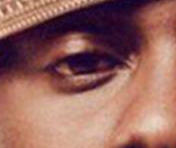
\includegraphics{tresZOOM.jpg}\newline
\caption{Imagen generada con kernel 3x3}
\end{center}\newline

%\subsubsection*{Detalle de la imagen con kernel 5x5}\newline
\begin{center}
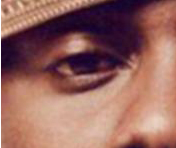
\includegraphics{cincoZOOM.jpg}\newline
\caption{Imagen generada con kernel 5x5}
\end{center}\newline\newline


%\subsubsection*{Detalle de la imagen con kernel 7x7}\newline
\begin{center}
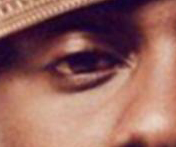
\includegraphics{sieteZOOM.jpg}\newline
\caption{Imagen generada con kernel 7x7}
\end{center}\newline
\newline

A pesar de que los cambios son sutiles, se puede observar que el efecto del filtro se incrementa, conforme el kernel se agranda. El kernel 7x7 crea un efecto borroso ligeramente más notorio que los otros dos kernel. \newline




\subsection{Experimento 3: mejora de tiempos de ejecución}

El algoritmo presentado en este documento (ver Algorithm 5), utilizado para aplicar un borrado gaussiano a una imagen, presenta una deficiencia en los tiempos de ejecución. A pesar de realizar el filtrado de la imagen con éxito, los tiempos de espera son, como se vio y se expondrá más adelante, relativamente largos y pueden entorpecer la experiencia final del usuario.\newline

El orden O grande del algoritmo es de $n^4$. Este orden elevado se presenta por la aparición de cuatro ciclos del tipo \for anidados. Al recorrer la imagen se recorre, también, el kernel utilizado, el cual se encuentra en forma matricial. Lo anterior da como resultado largos tiempos de ejecución.\newline

El objetivo de este apartado es mejorar el tiempo que le toma al algoritmo recorrer y modificar la imagen. Esto se realizará cambiando la manera en que se representa y se recorre el kernel utilizado. Además de variar el orden de un 5x5 a una matriz de tamaño 3x3.\newline

A continuación se muestra el algoritmo modificado:\newline

\begin{algorithm}
   \caption{Improved Gaussian Algorithm}
    \begin{algorithmic}[1]
      \Function{desaturation}{Bitmap bitmap }\\\Comment{Donde Bitmap es el el array de pixeles utilizados para programar en Android}
		\\
        \State int color, blue, green, red, sumBlue = 0, sumGreen = 0,				 \State sumRed = 0;
        \State  Bitmap image $= bitmap.copy(Bitmap.$
        \State $Config.ARGB8888, true)$
\\          
        
        

		\State $int[ ][ ] kernel =$
		\State \begin{bmatrix}
                1  & 2 & 1 \\
                2  & 4 & 2 \\
                1  & 2 & 1
                \end{bmatrix}
        \State int[] kernelX = new int[3];
        \State kernelX[0] = 4;
        \State kernelX[1] = 8;
        \State kernelX[2] = 4;

        \State int[] kernelY = new int[3];
        \State kernelY[0] = 4;
        \State kernelY[1] = 8;
        \State kernelY[2] = 4;
        
        \State int colorX, colorY, blueX, greenX, redX,
                blueY, greenY, redY;

         \State int imgH $= image.getHeight(); $
        \State int imgW $= image.getWidth(); $
       \State int kerL $= kernel.lenght; $
        
\\
        \For{$int y = 1;y<imgH-kL;y=y+1$}
            \For{$int x = 1;y<imgW-kL;x++$}
				%\For{$int v= 0; v < kL; v++$}
					\For{$int u= 0; u < kL; u++$}
					        \State colorX = image.getPixel(x+u, y); \Comment{Se recorre una fila}
                            \State colorY = image.getPixel(x, y+u);\Comment{Se recorre una columna}
						%\State color$= image.getPixel(x+u,y+v)$
						    \State blueX = Color.blue(colorX)
            				\State greenX = Color.green(colorX)
            				\State redX = Color.red(colorX)
            				
            				\State blueY = Color.blue(colorY)
            				\State greenY = Color.green(colorY)
            				\State redY = Color.red(colorY)
            				
            				\State sumGreen $+= (greenX)*kernelX[u]$
            				\State sumBlue $+= (blueX)*kernelX[u]$
            				\State sumRed $+= (redX)*kernelX[u]$
            				
            				\State sumGreen $+= (greenX)*kernelY[u]$
            				\State sumBlue $+= (blueX)*kernelY[u]$
            				\State sumRed $+= (redX)*kernelY[u]$
            			\EndFor
				%\EndFor
				\State sumGreen $=sumGreen/(kernelSum*2)$
				\State sumBlue $=sumBlue/(kernelSum*2)$
				\State sumRed $=sumRed/(kernelSum*2)$
				\State newImg = $ setPixel(x, y, $				
				\State Color.setRGB(Math.abs(sumRed), 
				\State Math.abs(sumGreen), Math.abs(sumBlue)));
        		\EndFor
        \EndFor
        \State return image
       \EndFunction

\end{algorithmic}
\end{algorithm}
\newpage

Para llegar al algoritmo anterior, se partió de la siguiente teoría: el kernel en forma de matriz se aplica en toda imagen. Dicho kernel posee filas y columnas con sus respectivos valores. El algoritmo anterior poseía dos ciclos \for para recorrer todo el kernel (filas y columnas). Se puede evitar uno de esos ciclos si se divide la matriz en una sola fila y una sola columna, cuyos elementos corresponden a la suma de todos los números de las filas o columnas que correspondan según su posición. Es decir, la posición primera del nuevo kernel 1x1 para el eje x corresponde a la suma de todos los números que están en la primera columna. Para la segunda posición, los números de la segunda columna. \newline

Por ejemplo,\newline
\begin{center}
                \begin{bmatrix}
                1  & 2 & 1 \\
                2  & 4 & 2 \\
                1  & 2 & 1
                \end{bmatrix}&
                
                \begin{bmatrix}
                (1+2+1)  & (2+4+2) & (1+2+1) \\
                \end{bmatrix}
                
                \newline
                
                =
                \begin{bmatrix}
                4  & 8 & 4 \\
                \end{bmatrix}
\end{center}               \newline

Una vez que se tiene la nueva matriz 1x1, se procede a recorrer las filas y las columnas por separado (de ahí las variables colorX y color Y). Se obtienen los valores RGB, se multiplican por el número indicado por la matriz nueva y se suman los valores. Por último, se divide el acumulado de todos los valores entre el doble de la suma de los números del kernel original y, de esta manera, se obtiene el color modificado.\newline

Estas modificaciones provocaron los siguientes resultados (tiempos en milisegundos):\newline


\subsubsection*{Gauss normal}\newline

Imagen 569x643\newline

25949, 26111, 26672, 26911, 26235.
\newline

Promedio: 26375.6\newline



\subsubsection*{Gauss modificado}\newline

Imagen 569x643\newline

14262, 14611, 14589, 14911, 14511.
\newline

Promedio: 14576.8








\begin{thebibliography}{1}

\bibitem{IEEEhowto:kopka}
H.~Kopka and P.~W. Daly, \emph{A Guide to \LaTeX}, 3rd~ed.\hskip 1em plus
  0.5em minus 0.4em\relax Harlow, England: Addison-Wesley, 1999.

\end{thebibliography}


\end{document}